\subsection*{Логическое следование формул}
\begin{definition}
    Формула $\Phi$ называется \textit{логическим следованием формул} $\Phi_1,\ldots,\Phi_m$, если при любой подстановке в эти формулы вместо их переменных $X_1,\ldots,X_n$ конкретных высказываний $A_1,\ldots,A_n$ из истинности высказываний $\Phi_1(A_1,\ldots,A_n),\ldots,\Phi_m(A_1,\ldots,A_n)$ следует истинность высказывания $\Phi(A_1,\ldots,A_n)$.

    Символическое обозначение $\Phi_1,\ldots,\Phi_m \models \Phi$ "--- называется \textit{логическим следованием}.

    Формулы $\Phi_1,\ldots,\Phi_m$ называются \textit{посылками} и формула $\Phi$ "--- \textit{следствием} логического следования $\Phi_1,\ldots,\Phi_m \models \Phi$.
\end{definition}

\begin{example}
    Докажем логическое следование:

    $F\Rightarrow G$, $K\Rightarrow \lnot H$, $H\lor\lnot G \models F\Rightarrow\lnot K$.
    
    Предположим противное:
    
        1. $F\Rightarrow G = 1$

        2. $K\Rightarrow\lnot H = 1$

        3. $H\lor\lnot G = 1$

        4. $F\Rightarrow\lnot K = 0$
    
    
    Из условия 4: $F = 1, \lnot K = 0, K = 1$.

    Из условия 1: $G = 1$, из условия 2: $\lnot H = 1, H = 0$.
    
    Значит, $H\lor\lnot G = 0$, что противоречит условию 3.

    Значит, предположение неверно и логическое следование выполняется.
\end{example}

\subsection*{Основные правила логического следования}
\begin{enumerate}
    \item \textit{Правило отделения} (или правило \textit{модус поненс} - от лат. modus ponens)
        $\Phi,\Phi\Rightarrow\Uppsi\models\Uppsi$

    \item \textit{Правило контрапозиции} 
    $\Phi\Rightarrow\Uppsi\models\lnot\Uppsi\Rightarrow\lnot\Phi$

    \item \textit{Правило цепного заключения} 
    $\Phi_1\Rightarrow\Phi_2,\Phi_2\Rightarrow\Phi_3\models\Phi_1\Rightarrow\Phi_3$
    \item \textit{Правило перестановки посылок} 
    $\Phi_1\Rightarrow(\Phi_2\Rightarrow\Phi_3)\models\Phi_2\Rightarrow(\Phi_1\Rightarrow\Phi_3)$
\end{enumerate}

\begin{definition}
    Множество формул $\Phi_1,\ldots,\Phi_m$ называется \textit{противоречивым}, если из него логически следует любая (в том числе и тождественно ложная) формула $\Phi$.

    Символически это записывается $\Phi_1,\ldots,\Phi_m\models $.

    В противном случае множество формул $\Phi_1,\ldots,\Phi_m$ называется \textit{выполнимым}.
\end{definition}

\begin{lemma}[Критерии логического следования]
    Условие $\Phi_1,\ldots,\Phi_m\models \Phi$ равносильно каждому из следующих условий:
    \begin{enumerate}
        \item $\Phi_1\land\ldots\land\Phi_m\models\Phi$
        \item $\models \Phi_1\land\ldots\land\Phi_m\Rightarrow\Phi$
        \item $\Phi_1,\ldots,\Phi_m,\lnot\Phi\models$
    \end{enumerate}

В частности, $\Phi\models\Uppsi$ равносильно $\models\Phi\Rightarrow\Uppsi$.
Отсюда также следует, что $\Phi=\Uppsi$ равносильно тому, что $\Phi\models\Uppsi$ и $\Uppsi\models\Phi$.
\end{lemma}

Вывод: следующие задачи равносильны:
\begin{enumerate}
    \item Проверка тождественной истинности формул
    \item Проверка логического следования формул
    \item Проверка тождественной ложности формул
    \item Проверка противоречивости множества формул
\end{enumerate}
\subsection*{Методы проверки тождественной истинности формул}
Основные методы проверки тождественной истинности формул:
\begin{enumerate}
    \item Прямой метод
    \item Алгебраический метод
    \item Алгоритм Квайна
    \item Алгоритм редукции
    \item Метод семантических таблиц
    \item Метод резолюций
\end{enumerate}
\subsection*{Алгебраический метод}
\textit{Алгебраический метод} преобразования формулы $\Phi = \Phi(X_1,\ldots,X_n)$ с помощью равносильных преобразований в тождественно истинную формулу 1.
\begin{example}
    С помощью равносильных преобразований выяснить, является ли тождественно истинной формула

$\Phi = ((Y\Rightarrow Z)\land(X\Rightarrow V)\land(X\lor \lnot Z))\Rightarrow(\lnot Y\lor V) \\ = 
\lnot((\lnot Y \lor Z)\land(\lnot X\lor V)\land(X\lor \lnot Z))\lor(\lnot Y\lor V) \\ =
((Y\land\lnot Z)\lor(X\land\lnot V)\lor(\lnot X\land Z))\lor\lnot Y \lor V \\ = 
((Y\land\lnot Z)\lor\lnot Y)\lor((X\land\lnot V)\lor V)\lor (\lnot X\land Z) \\ =
((Y\lor\lnot Y)\land(\lnot Z\lor\lnot Y))\lor((X\lor V)\land(\lnot V\lor V))\lor (\lnot X\land Z) \\ =
\lnot Z\lor\lnot Y\lor V\lor(X\lor(\lnot X\land Z)) \\ = 
\lnot Z \lor \lnot Y \lor V\lor ((X\lor \lnot X)\land(X\lor Z)) \\ =
\lnot Z\lor\lnot Y \lor V \lor X \lor Z \\ = 
(Z \lor \lnot Z)\lor\lnot Y\lnot V\lnot X = 1$.
\end{example}

\begin{remark}
    Если в процессе упрощения исследуемой формулы не получилась тождественно истинная формула 1, то следует попытаться подобрать значения пропощициональных переменных, при которых истинностное значение формулы равно 0.
    Это докажет,  что исследуемая формула не является тождественно истинной.
\end{remark}

\subsection*{Алгоритм Квайна}
\textit{Алгоритм Квайна} позволяет сократить полный перебор значений пропозициональных переменных за счет последовательного фиксирования возможных значений 0 или 1 пропозициональных переменных и последующего анализа истинностных значений полученных формул с меньшим числом переменных.

\begin{figure}[H]
    \centering
    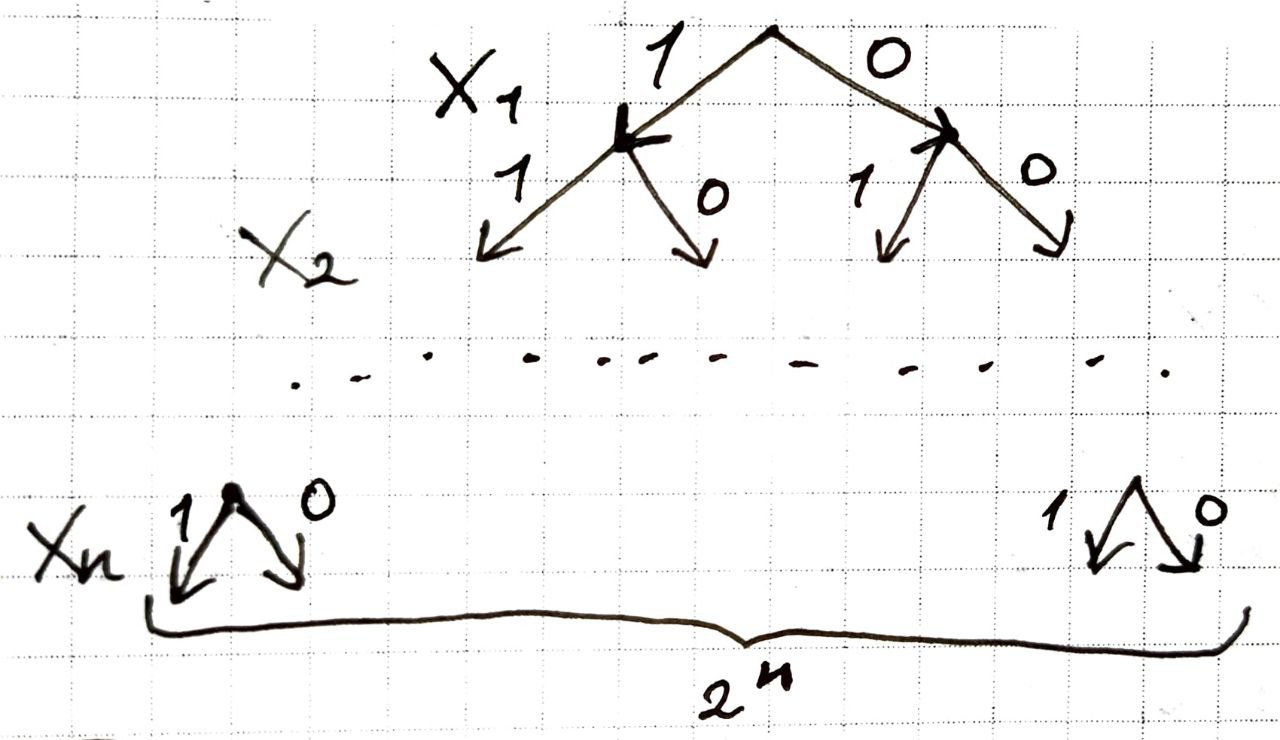
\includegraphics[height = 4cm]{images/kvain.jpg}
    \caption{Дерево перебора значений переменных}
\end{figure}

При этом используются основные тавтологии и следующие простейшие равенства:

$X\land1 = X$ \qquad $X\lor 1 = 1$ \qquad $0\Rightarrow X = 1$ \qquad $X\Rightarrow X = 1$

$X\land 0 = 0$ \qquad $X\lor 0 = X$ \qquad $1\Rightarrow X = X$ \qquad $X\Leftrightarrow X = 1$

$X\land\lnot X = 0$ \quad $X\lor\lnot X = 1$ \qquad $X\Rightarrow 1 = 1$  \qquad $X\Rightarrow 0 = \lnot X$

\begin{example}
    C помощью алгоритма Квайна выясните, является ли тождественно истинной формула
    $((Y\Rightarrow Z)\land(X\Rightarrow V)\land(X\lor\lnot Z))\Rightarrow(\lnot Y \lor V)$.

    1. При фиксировании в исходной формуле $X = 1$ получаем 
    
    $((Y\Rightarrow Z)\land(1\Rightarrow V)\land(1\lor\lnot Z))\Rightarrow(\lnot Y \lor V)$, что равносильно 
    
    $((Y\Rightarrow Z)\land V)\Rightarrow (\lnot Y\lor V)$.

    Положим здесь $Y = 1$: $((1\Rightarrow Z)\land V)\Rightarrow (\lnot 1\lor V)$, 
    
    что равносильно $(Z\land V)\Rightarrow V$.

    Отсюда при $Z = 1$ получаем $(1\land V)\Rightarrow V = V \Rightarrow V = 1$

    и при $Z = 0$ получаем $(0\land V)\Rightarrow V = 0 \Rightarrow V = 1$.

    Положим теперь $Y = 0$: $((0\Rightarrow Z)\land V)\Rightarrow(\lnot 0 \lor V) = V \Rightarrow 1 = 1$.
\\ \\
    2. При фиксированном в исходной формуле $X = 0$ получаем 

    $((Y\Rightarrow Z)\land(0\Rightarrow V)\land(0\lor\lnot Z))\Rightarrow(\lnot Y \lor V)$, что равносильно 
    
    $((Y\Rightarrow Z)\land\lnot Z) \Rightarrow (\lnot Y \lor V)$.

    Положим здесь $Y = 1$: $((1\Rightarrow Z)\land\lnot Z)\Rightarrow(\lnot 1 \lor V)$, что равносильно 
    
    $(Z\land\lnot Z)\Rightarrow V = 0 \Rightarrow V = 1$.

    Положим теперь $Y = 0$: $((0\Rightarrow Z)\land\lnot Z)\Rightarrow(\lnot 0\lor V)=\lnot Z \Rightarrow 1 = 1$.

    Таким образом, данная формула тождественно истинная.
\end{example}

Т.е. метод решения заключается в том, что для входящих в формулу пропозициональных переменных последовательно фиксируются возможные значения 0 или 1, и получившиеся формулы упрощаются с помощью перечисленных ранее простейших равенств до тех пор, пока не получается тождественно истинная формула 1.

При этом порядок фиксирования значений пропозициональных переменных может быть произвольным.

\begin{remark}
    Если на каком-то заключительном шаге вычислений получается не тождественно истинная формула 1, а тождественно ложная формула 0, то исследуемая формула не является тождественной истинной "--- она опровергается соответствующими фиксированными значениями пропозициональных переменных. 
\end{remark}

\subsection*{Алгоритм редукции}
\textit{Алгоритм редукции} используется при доказательстве тождественной истинности формулы с большим количеством импликаций. 

Идея метода основывается на получении противоречия из предположения, что истинное значение рассматриваемой формулы равно 0 при некоторых истинностных значениях ее пропозициональных переменных. 

При этом используется тот факт, что импликация ложна в том и только том случае, если ее посылка истинна и заключение ложно. 

\begin{example}
    С помощью алгоритма редукции выяснить, является ли тождественно истинной формула

    $((Y\Rightarrow Z)\land(X\Rightarrow V)\land(X\lor\lnot Z))\Rightarrow(\lnot Y\lor V)$.
    
    \textit{Решение.} Запишем по пунктам шаги алгоритма редукции.

    1. Предположим, что при некотором наборе значений переменных данная формула ложна, т.е. выполняется
$((Y\Rightarrow Z)\land(X\Rightarrow V)\land(X\lor\lnot Z))\Rightarrow(\lnot Y\lor V) = 0$, т.е. последняя импликация в ней ложна.

    2. По определению операции импликации это равносильно тому, что посылка импликации $(Y\Rightarrow Z)\land(X\Rightarrow V)\land(X\lor\lnot Z) = 1$ и ее следствие $\lnot Y\lor V = 0$.

    3. По определению операций конъюнкции и дизъюнкции это равносильно тому, что $Y\Rightarrow Z = 1$, $X\Rightarrow V = 1$, $X\lor\lnot Z = 1$ и $\lnot Y = 0$, $V = 0$.

    4. Отсюда по определению операции отрицания получаем, что $Y = 1$.
    
    5. Тогда по определению операции импликации из первого равенства пункта 3 следует $Z = 1$ и из второго равенства этого пункта следует $X = 0$.

    6. Отсюда по определению операции отрицания получаем, что $\lnot Z = 0$.

    7. Подставляя найденные значения $X = 0,\lnot Z = 0$ в формулу $X\lor\lnot Z$, по определению операции дизъюнкции получаем условие $X\lor\lnot Z = 0$, которое противоречит третьему равенству пункта 3.

    Значит, наше предположение неверно и данная формула является тождественно истинной.
\end{example}

\begin{figure}[H]
    \centering
    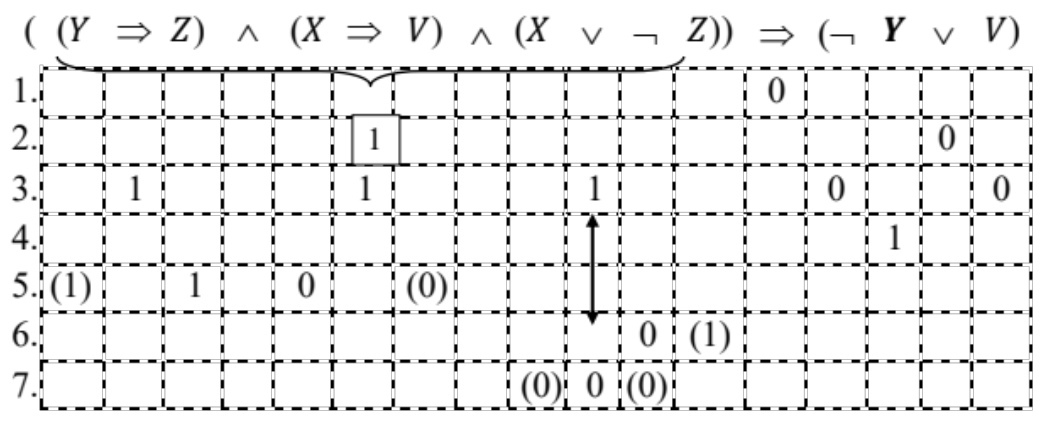
\includegraphics[height = 3cm]{images/reducto.jpg}
    \caption{На каждом шаге алгоритма в скобках указываются значения переменных, которые были получены ранее на предыдущих шагах вычислений}
\end{figure}

\subsection*{Метод семантических таблиц в алгебре высказываний}
\begin{definition}
    \textit{Оценкой переменных} в формуле $\Phi = \Phi(X_1,\ldots,X_n)$ называется отображение $\alpha$ множества $\{X_1,\ldots,X_n\}$ в множестве $\{0,1\}$.
    Обозначения: $\models_a\Phi$ и $\nvDash_a \Phi$.
\end{definition}
\begin{definition}
    \textit{Семантической таблицей} называется упорядоченная пара множества формул $\langle\Gamma |\Delta  \rangle $.

    Семантическая таблица $\langle\Gamma |\Delta  \rangle $ называется \textit{выполнимой}, если существует такая оценка переменных $a$, что
    \begin{enumerate}
        \item $\Phi\models_a$ для любой формулы $\Phi \in \Gamma$
        \item $\Uppsi\nvDash_a$ для любой формулы $\Uppsi\in\Delta$
    \end{enumerate}
\end{definition}

\begin{example}
    Семантическая таблица $\langle \{X,\lnot Y\} | \{X\Rightarrow Y\} \rangle $ выполнима для оценки $a(X) = 1, a(Y) = 0$.
\end{example}

\begin{example}
    Семантическая таблица $\langle \varnothing | \{X \lor\lnot X\} \rangle $ невыполнима.
\end{example}

\begin{theorem}[Основная теорема метода семантических таблиц]
    Для любой формулы $\Phi$ условие $\models \Phi$ выполняется тогда и только тогда, когда семантическая таблица $\langle \varnothing | \{\Phi\} \rangle $ невыполнима.
\end{theorem}

\begin{example}
    С помощью семантических таблиц докажем тождественную истинность формулы $\Phi = ((X\Rightarrow Y)\Rightarrow X)\Rightarrow X$, которая называется \textit{законом Пирса}.
\end{example}

Табличный вывод семантической таблицы $T_0 = \langle \varnothing | \Phi \rangle $:
\begin{figure}[H]
    \centering
    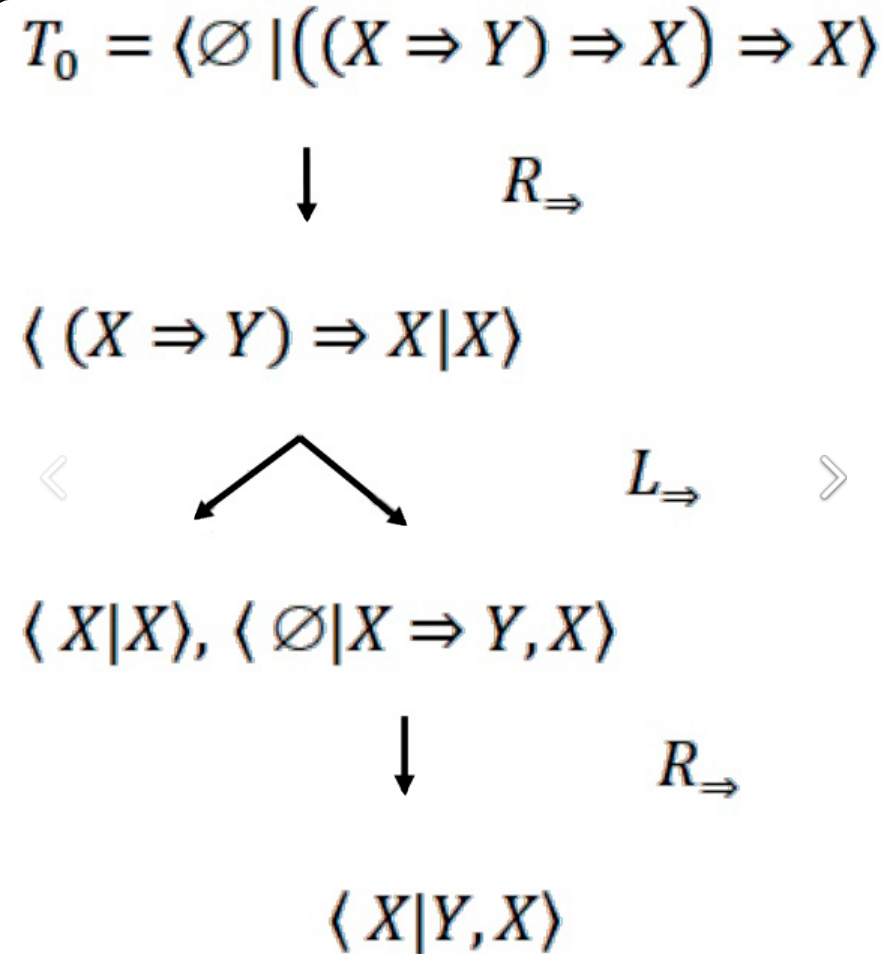
\includegraphics[height = 4cm]{images/pirse.png}
\end{figure}

(Про эти штуки есть еще немного в конспектах, но в целом зачем?..)
